\documentclass{scrreprt}
\usepackage{hyperref}
\usepackage[dutch]{babel}
\usepackage{graphicx}
\usepackage{etoolbox}
\usepackage{float}

%Remove newpage from chapter
\makeatletter
\patchcmd{\scr@startchapter}{\if@openright\cleardoublepage\else\clearpage\fi}{}{}{}
\makeatother
\DeclareGraphicsExtensions{.pdf,.png,.jpg}

\title{SOP6 Dynamic Software Quality}
\author{Guus Hamm en Rick Rongen}
\date{\today}

\begin{document}
	\maketitle
	\tableofcontents
	\newpage
	\chapter{Dynamische eigenschappen}
	Voor het bepalen van de kwaliteit van onze software zijn een aantal zaken belangrijk. Voor ons project zal zich dit vooral focussen op performance, en op robuustheid. Dit omdat dit voor het te monitoren systeem belangrijke eigenschappen zijn. Het is voor ons systeem van belang dat het beschikbaar is aangezien het een mission critical systeem is. Voor het meten van deze statistieken kan gebruik gemaakt worden van influxdb. Influxdb heeft meerdere meetpunten waarvan deze gegevens bij houd. Denk hierbij bijvoorbeeld aan disk reads per seconde, het aantal server request gemapped op de hoeveelheid cpu usage, het aantal SQL queries of de lading op de database. Door deze statistieken te koppelen aan een dashboard als Grafana worden de dynamische eigenschappen duidelijk.
	\begin{figure}[ht]
		\centering
		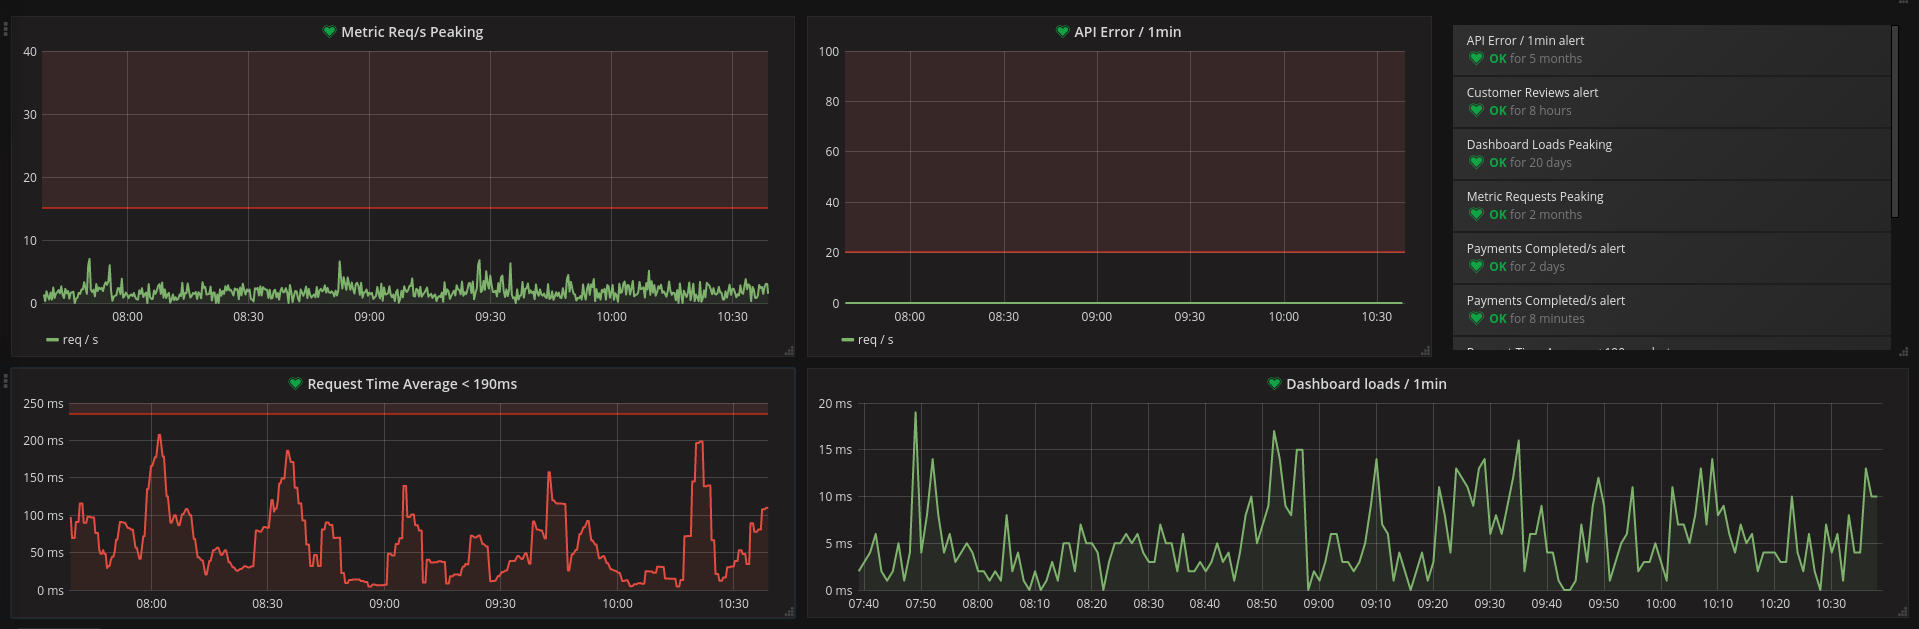
\includegraphics[width=\linewidth]{grafna-influxdb.png}
		\label{fig:grafana&influxdb}
		\caption{Grafan and Influxdb}
	\end{figure}
	
	In figuur \ref{fig:grafana&influxdb} is een Grafana te zien die is ingesteld om een alert te geven indien een waarde boven een threshold komt. Dit is een oplossing die wij ook kunnen gaan toepassen op ons project. Grafana bied de mogelijkheid om bij een alert een webhook af te vuren. Dit zou geïntegreerd kunnen worden met Jenkins om bij het uitvoeren van een build te controleren of de belasting van de server of het aantal fouten in de api bij het uitvoeren van de code te testen. Grafana zal geïntegreerd worden met Gerrit. Hierdoor wordt het direct duidelijk wat de stabiliteit van de software is.
\end{document}